%%%%%%%%%%%%%%%%%%%%%%%%%%%%%%%%%%%%%%%%%%%%%%%%%%
%	DISSERTATION CHAPTER CONVERSION STEPS 
%%%%%%%%%%%%%%%%%%%%%%%%%%%%%%%%%%%%%%%%%%%%%%%%%%
%	Remove everything above here
%	Remove \end{document}
%	Remove appendix, bibliography
\chapter[Chapter 1]{Post-Shooting Policing Evidence of Reduced Intensity and Effectiveness in Traffic Stops}
\addcontentsline{lof}{chapter}{\numberline{\thechapter}Chapter 1}
\addcontentsline{lot}{chapter}{\numberline{\thechapter}Chapter 1}
%	overwrite ``chapter1'' file 

\graphicspath{{C:/Users/david/coding/02_TRAFFIC_BIAS_paper/6000_LaTeX/figures/}}

%%%%%%%%%%%%%%%%%%%%%%%%%%%%%%%%%%%%%%%%%%%%%%%%%%
%	INTRODUCTION 
%%%%%%%%%%%%%%%%%%%%%%%%%%%%%%%%%%%%%%%%%%%%%%%%%%
\section{Introduction} 
%	What is the motivation? 
Minority drivers receive differential treatment from law enforcement officers (LEO) in the U.S. (Mewkawi \& Breslin, JESP 2015), they are more likely to be shot (Khan \& Davies, JSI 2017), and they are treated with less respect (Voigt et al, NAS 2017). According to recent Pew Center surveys of Americans (2016, 2019), both black and white respondents say that black citizens are treated less fairly both by police and by the justice system, with 59\% for black men and 31\% for black women respondents, black adults are 5x more likely to say that they have been unfairly stopped by the police relative to their white counterparts, and across various metrics black Americans are far less likely than white to approve of the way that police do their jobs. \\

%	Why does it matter? 
Studying racial disparities in policing can bring many potential benefits, including a better understanding of patterns and systemic failures, increased accountability over police who innately hold a position of power, the development of more effective training and interventions, and fostering stronger public trust stemming from fairer policing practices. \\

%	What are my questions? 
This paper seeks to explore the response patterns of police officers and drivers following a fatal police encounter. Do police departments change their traffic stop behaviors after fatally shooting an unarmed black person? Do these behaviors change in a way that differs across race? Does policing intensity or effort level change following a lethal shooting? Do these patterns change differently when an event receives national scrutiny? \\ 

%	Why is this needed? 
These questions are made difficult to answer not only due to the lack of consistent, publicly-available policing data, but also by the relatively infrequent nature of an officer-involved unarmed death, and by the highly-sensitive timing of these events across the years. I address these issues by combining subject-death information; the most severe police-civilian interaction, with traffic stop data; the most frequent at 50,000 per day, using the largest data sets available. \\

%	What do I do? 
I begin by merging the Stanford Open Policing Project (SOPP) and Fatal Encounters (FE) data sets to closely consider the exact date of traffic stops and searches surrounding these momentous deaths and to look closely for observable changes in behavior. I am able to observe black vs overall stops, searches, and search successes (hits) and I am further able to combine these measures into rate-based metrics which carry meaningful and less-direct interpretations. Using this novel, detailed data combination, I leverage the exogenous timing of a fatal police encounter and run a series of volume-based and rate-based difference-in-difference regressions, heterogeneity analyses by public scrutiny level, and corresponding event studies to address my research questions. \\

%	What do I find? 
My primary causal finding is a large decrease in stop volumes, both overall and for black drivers, implying that police are decreasing their efforts on the front-end following a death event, with subsequent significant decreases in search and hit volumes. By splitting events across publicity levels, I explore heterogeneous effects, finding suggestive evidence that this decrease in efforts is largest when event scrutiny is low. My causal results appear to be driven by low scrutiny events, whereas for high scrutiny events there is a pattern of decreasing black hit rates and black-shares of hits, indicating that scrutiny may alter policing decisions. \\

%	What does this mean? 
Taken together, my findings indicate that traffic stop patterns change following a death event in a way that would be consistent with decreased policing effort across-the-board. These reductions imply either a behavioral or institutional response by officers and departments following a death event, consistent with either individual officer apprehension or risk aversion, or changes in departmental policy or directives, or political pressure. These volume decreases may be driven by low scrutiny events, indicating that public spotlight could affect these effort patterns, and further suggesting that traffic stop reductions are driven by police-side changes, when the public awareness levels are low. \\

%	What do others do? 
In the existing literature, it has been shown that white LEOs are more likely to use force in minority neighborhoods (Hoekstra \& Sloan, AER 2022). Minority drivers are treated differently as well; they are given fewer discretionary ``discounts" (Goncalves \& Mello, AER 2021), officers are more likely to stop black drivers following a Trump campaign rally (Grosjean, Masera \& Yousef, QJE 2022), black drivers' cars are more likely to be searched (Knowles, Persico \& Todd, JPE 2001), and police have a lower inferred-threshold for searching minority drivers (Pierson et al, 2020). \\

%	How am I different? 
This paper expands upon the preexisting literature by casting a wider net, with findings holding across multiple departments, events and years. I also enact a more rigorous analysis than in previous efforts to measure police responses to fatal shootings (Powell 2023). By introducing internet search data, I consider a new dimension of the problem - national scrutiny.  \\

%	What is my contribution? 
Each death-event that I analyze is significant. Cumulatively, deaths by police account for 5\% of all homicides in the US (Ang \& Tebes, APSR 2023) and are garnering increased levels of public attention. In addition to the intrinsic importance of a human life, there is public value that comes from good policing which demands public trust and accountability. To my knowledge, this is the first paper to consider such a large set of unarmed civilian death events, and it is the first paper to utilize public scrutiny levels to explore heterogeneous treatment patterns. As these deaths continue and gain widespread exposure, it is becoming more and more crucial for good governance to analyze these events and their aftermaths, both to better understand policing responses, as well as to avoid exacerbating tumultuous events further. 

%%%%%%%%%%%%%%%%%%%%%%%%%%%%%%%%%%%%%%%%%%%%%%%%%%
%	THEORETICAL CONSIDERATIONS 
%%%%%%%%%%%%%%%%%%%%%%%%%%%%%%%%%%%%%%%%%%%%%%%%%%
\section{Theoretical Considerations} 
%	Basic Setup: 
Before making a traffic stop, a police officer observes a set of signals from a driver and their vehicle, and use this information to determine whether or not to make a stop; were they speeding, did they run a light, etc.. During the stop, a similar process is repeated where the officer receives more specific signals. They consider day of week, time of stop, and location, but they also observe idiosyncratic driver characteristics such as perceived race, gender, and other intangibles like nervousness, sobriety, and the general demeanor of the driver and their passengers. After receiving this set of signals, the officer considers the likelihood that the vehicle is carrying contraband and determines whether or not to conduct a search which may yield contraband, resulting in a hit. \\

From the previous literature, this hit rate may then be thought of as the officer's expected likelihood of finding contraband during a search. At one extreme, if a department only searches vehicles when they are certain of contraband, their hit rate will approach 100\%. On the other end, if a department searches vehicles at random, their hit rate will approach the underlying contraband-carrying rate of the driving population. \\

In order to evaluate the questions of this study, I first consider the wake of any officer-involved fatal black shooting to explore changes in policing patterns, and then I split these events based on public scrutiny levels in efforts to explore differential patterns when the American public is watching closely, and when they are not, to separate underlying incentives of the observed patterns. \\

Consider policing incentives which my departmental data is more equipped to address. Officers may feel a lack of appreciation from the public, the inherent risk of their job may become more salient, or the possibility that they must choose to shoot or not shoot a civilian may become more relevant. The department itself may urge officers to be more cautious and deliberate, they may need to reallocate their limited resources to address protests or conduct internal reviews, or they may receive political- or media-based pressures. These lines of thought generally predict decreases in policing intensity due to individual officer behavioral changes or institutional policies and directives. \\

Turning to civilian incentives, which I am less able to assess, it is ambiguous whether there will be more or less drivers on the road. On one hand, drivers may going to or from protests. On the other hand, they may grow fearful of police violence and reduce their chances for police interaction by avoiding driving, more carefully adhering to traffic laws, or choosing not to carry contraband. Taken together, these incentives give an ambiguous prediction. \\

Examining my scrutiny-based results, I am able to speak to some of these concerns about police vs driver-side responses, although I advise against causal interpretations due to endogeneity concerns with inferred public scrutiny levels. I find that the overall volume decreases are strongest for low scrutiny events, while for high scrutiny events I instead find lower black shares of hits and hit rates. These findings carry implications about public information sets, as civilians are less likely to be aware of the shooting or its details at all, suggesting that observed volume decreases are likely driven by police-side responses, while for more infamous shootings, the risk of police confrontation may grow and drivers have further incentive to avoid carrying contraband. \\

Further, non-publicized events create internal pressure and feel more personal to the department, while those which receive national attention receive external pressures and may be perceived as more political or more removed for individual officers. This suggests that on the stop margin, staff disruptions and risk aversion may be more likely mechanisms for discretionary stop decreases under low scrutiny. When an event receives widespread attention, external forces and politics come into play and may dictate that officers maintain appearances, stabilizing front-end stop behaviors, and opening up the possibility of a department receiving additional resources to mitigate increases in resource demands for reporting procedures or protest responses, consistent with smaller or insignificant policing intensity decreases under national attention. \\

Finally, for high scrutiny events, which I again urge caution against direct causal interpretations, it becomes ambiguous whether reductions in black hit rates and shares are driven by police- or civilian-side behaviors. Black drivers afraid of lethal confrontation have incentive not to carry contraband, and police fearing political or external repercussions have incentive to reduce confrontations which may exacerbate the situation further too. In future research, these important questions may be reevaluate and better addressed. \\

%%%%%%%%%%%%%%%%%%%%%%%%%%%%%%%%%%%%%%%%%%%%%%%%%%
%	DATA DESCRIPTION 
%%%%%%%%%%%%%%%%%%%%%%%%%%%%%%%%%%%%%%%%%%%%%%%%%%
\section{Data}
For this paper, I use three data sources. The Stanford Open Policing Project (SOPP), Fatal Encounters (FE), and Google Trends, which I break down in further detail below. \\

%	SOPP Data: 
\subsection{The Stanford Open Policing Project: Traffic Stop Data}
The SOPP data consists of traffic stop information for 88 locales throughout the contiguous U.S. which were acquired via Freedom of Information Act (FOIA) requests by a team of Stanford researchers which I then cleaned and appended together. This data has been used in a number of prominent papers, such as Grosjean, Masera \& Yousef (QJE 2022), and serve as the best-available traffic stop data to date, with figure \ref{sopp_map} depicting the relevant SOPP data coverage. \\

%	SOPP Data Map: 
\begin{figure}
	\begin{center}
		\includegraphics[width=6.0in]{stop_data_map.eps}
		\caption[Traffic Stop Data Map]{This map shows traffic stop data availability from the SOPP data set. States with both state patrol + full jurisdictional data are in dark gray, states with only state patrol data in light gray, and states with no statewide data in white, with red dots corresponding to municipal data, are scaled to the number observations available.}
		\label{sopp_map}
	\end{center}
\end{figure}

To clean the data, I de-duplicate the four overlapping-jurisdictions in the data, (e.g. Chicago, IL vs Statewide Illinois). An issue arose with unreliable department-naming practices in the SOPP data, forcing me to manually search and rename departments for consistency and to allow a later merge with the Fatal Encounters data. I manually looked for the actual name for each department changed them to align with Fatal Encounters conventions, e.g. ``LMPD" and ``Louisville Metro PD" were changed to ``Louisville Metro Police Department". \\

As this analysis relies heavily on event-timing, I drop a number of departments that only reported stop data at the monthly or annual level. If a department always reported stops on the same day of each month, these were identified as ``monthly reporters" and dropped, similarly for ``annual reporting" departments. \\ 

After this, following conventions from existing literature, I drop pedestrian stops from the analysis, as I am focusing on traffic behaviors. I also drop ``consent" and ``plain view'' searches, again following the existing literature, as these are inherently different as either explicit permission (consent) or direct officer line-of-sight (plain view) largely alter the discretionary component of the officer search decision. \\

Lastly, as my analysis relies on driver race as well as search and hit information, I implement a flexible filtration approach to determine ``reliability'' of race, search, and hit data recording. I consider at the overall black rate for stops in my data set (4.4\%), and look for time periods where each department records at least $1/(4.4\%/20)=465$ stops, if none of these stops were recorded as black, I consider the department an unreliable reporter for the corresponding period. This is done in a wide-to-narrow manner, starting with the entire time frame, then checking each year, month, and week - where for large departments recording 465+ stops in a week, none of which are black, I remove that week from my data. In this way I only consider departments which \textit{reliably} record the pertinent data. \\

%	FE Data: 
\subsection{Fatal Encounters: Event Timing Data}
Beginning in 2012, the Fatal Encounters began collecting information on police-killings in the U.S. with a team of volunteer researchers via FOIA requests, scouring newspaper articles, and crowd-sourced submissions which were checked and added to the database. Their stated goal is to construct an ``impartial, comprehensive, searchable national database of people killed during interactions with the police'', back-collecting data going back to 2000. As it stands, this is the most-reliable source of officer-involved-death information in the United States. When compared with either government sources (Finch et al, 2019) or with alternative open-source data sources (Renner, 2018), Fatal Encounters has been shown to both be more reliable and more comprehensive. \\

Starting from a basic data download of nearly 31,500 deaths, I choose a limited sub-sample of these deaths to capture a specific type of event for my analysis. Citizen weapon possession is the most consistent predictor of police usage of deadly force (Mora, Terrill \& Foster, 2022) and as such, I use only \emph{unarmed} deaths in this study. This limits my analysis to deaths where I have information about subject-armedness, leaving only the 2011-2018 period, reducing my potential events to 17,149, out of which 6,128 subjects were listed as unarmed. Next, I am interested in black deaths as per my research question, of which there remain 1,814. After this I consider only shooting/bludgeoning/asphyxiation deaths where direct and potentially-lethal force was used, as opposed to deaths with less-direct lethal intent, e.g. car crashes, drownings, lethal falls, leaving me with 610 events. \\

After merging, I manually look into each of the matched-deaths to pinpoint precisely which department caused each death, to confirm specific death timings, and to verify that the nature of each death is consistent with the goals of my study; excluding things like murder-suicides, hostage situations, and one prolonged escaped-prisoner manhunt. I am left with 78 matched-focal-events with suitable pre- and post-event SOPP traffic data for my full analysis (relegated to the appendix). In what follows, I balance the data using pre- and post-period observations, leaving 28 usable events.  \\

%	Google Trends Data: 
\subsection{Google Trends: Public Scrutiny Data}
In order to assess whether public attention influences traffic stop behaviors, a proxy was required to infer scrutiny levels for each subject-death. Following from the ``Say Their Names" movement that began and grew throughout much of my sample, I pulled internet search information using Google Trends. As the website only gives relative-volumes, I required a benchmark event to scale search rates and allow comparisons. I chose the most-searched name in my time period and its corresponding department - Michael Brown and the Ferguson Police Department to determine relative-search-frequencies. \\

After converting relative search trends to the same comparable standard for my focal events, I measure the increase in pre- vs post-event average scrutiny levels, and I take the difference in the two to separate events into low- vs high-scrutinies using pre- and post-event means to maintain robustness. If the mean-change in searches for a person's name is very low relative to Michael Brown's, I consider their death not to be scrutinized, and if the difference is large, I consider it to be highly-scrutinized. 

%%%%%%%%%%%%%%%%%%%%%%%%%%%%%%%%%%%%%%%%%%%%%%%%%%
%	METHODOLOGY & RESULTS 
%%%%%%%%%%%%%%%%%%%%%%%%%%%%%%%%%%%%%%%%%%%%%%%%%%
\section{Methodology \& Main Results}
For the purposes of this paper a specific type of death is used to define a department's treatment status - one of their officers must be observed fatally shooting, bludgeoning, or asphyxiating an unarmed black subject. Each traffic stop is then assigned an ``event time" based on the number of days to the nearest event. As a result, any department with multiple observed-events has each of its traffic stop dates matched to the \textit{nearest} event date, as demonstrated in Figure \ref{etime_diagram}. \\

%	Event Time Diagram: 
\begin{figure}
	\begin{center}
		\noindent \underline{-Single-Event Departments} \\
		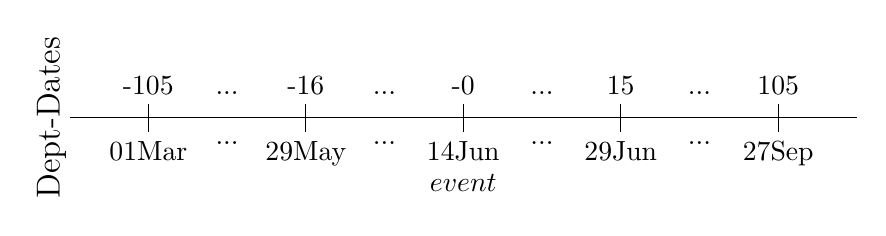
\begin{tikzpicture}
			\draw (0,0) -- (10,0);
			\foreach \x in {1, 3, 5, 7, 9}
			\draw (\x, 5pt) -- (\x, -5pt);
			\draw (1,0) node[below=5pt] {01Mar} node[above=5pt] {-105};
			\draw (3,0) node[below=5pt] {29May} node[above=5pt] {-16};
			\draw (5,0) node[below=5pt] {14Jun} node[above=5pt] {-0};
			\draw (5,0) node[below=17pt] {$event$};
			\draw (7,0) node[below=5pt] {29Jun} node[above=5pt] {15};
			\draw (9,0) node[below=5pt] {27Sep} node[above=5pt] {105};
			\foreach \y in {2, 4, 6, 8}
			\draw (\y,0) node[below=5pt] {...} node[above=5pt] {...};
			\path (0,0) -- (10,0) node[rotate=90,midway,sloped,above=140] {\large Dept-Dates};
		\end{tikzpicture} \\
		\underline{-Multi-Event Departments} \\
		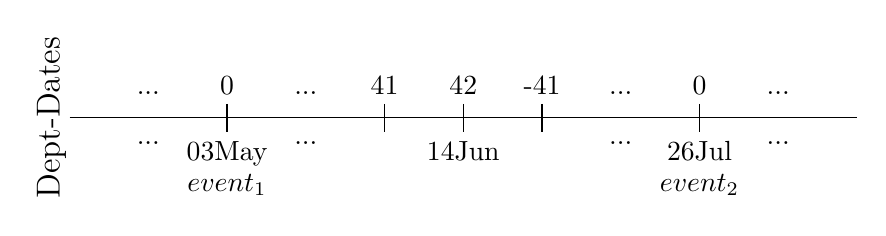
\begin{tikzpicture}
			\draw (0,0) -- (10,0);
			\foreach \x in {2, 4, 5, 6, 8}
			\draw (\x, 5pt) -- (\x, -5pt);
			\draw (2,0) node[below=5pt] {03May} node[above=5pt] {0};
			\draw (2,0) node[below=17pt] {$event_{1}$};
			\draw (4,0) node[above=5pt] {41};
			\draw (5,0) node[below=5pt] {14Jun} node[above=5pt] {42};
			\draw (6,0) node[above=5pt] {-41};
			\draw (8,0) node[below=5pt] {26Jul} node[above=5pt] {0};
			\draw (8,0) node[below=17pt] {$event_{2}$};
			\foreach \y in {1, 3, 7, 9}
			\draw (\y,0) node[below=5pt] {...} node[above=5pt] {...};
			\path (0,0) -- (10,0) node[rotate=90,midway,sloped,above=140] {\large Dept-Dates};
		\end{tikzpicture}
		\caption[Event Timing Dragram]{The above demonstrates how event-times are defined relative to event-dates for a representative single- and multi-event department.}
		\label{etime_diagram}
	\end{center}
\end{figure}

%Following from Becker (1957, 1993), particular attention is placed on the post-decision hit-rate outcome. 
Following from the work of Grosjean, Masera \& Yousef (QJE 2023), this paper then collapses individual traffic stop observations to the department-date level. From here, I have six volume outcomes that I consider, total stop volume and black stop volume, total search volume and black search volume, total hit volume and black hit volume. Next, I utilize share outcomes to analyze whether changes in volumes are disproportionately-black. The black stop share measures the black-proportion of traffic stops, and changes here would indicate that black vs non-black stop volume changes are outpacing one another. Similarly for searches, I consider the black search share which measures the black-proportion of searched vehicles, and for hits the black hit share measures the black-proportion of hits. \\

I further consider rate outcomes which might be thought of as post-stop decision probabilities. The black search rate measures how frequently stopped black drivers are searched, the hit rate measures how frequently the searches prove successful and, as previously discussed, speaks to the expected contraband carrying rate that an average officer from each department has when making a search decision. Finally, I consider the black hits-to-stops ratio which measures how frequently black drivers are found with contraband on a per-stop basis. \\

Each of the above six volume outcomes, three share outcomes, and three rate outcomes are used in the equations to follow. I first run difference-in-differences with corresponding event studies, as described in equations \ref{eq1_DiD} and \ref{eq2_estudy}. 

%	Raw Differences in Outcomes
\begin{center}
	\input{C:/Users/david/coding/02_TRAFFIC_BIAS_paper/6000_LaTeX/tables/descriptive_statistics_main_full}
\end{center}

%	Equation #1, Difference in Differences
\begin{equation}
	\begin{split}
		Y^{o}_{d,t} = \beta Post_{d,t} + \boldsymbol{X'}_{d,t} \boldsymbol{\gamma} + \boldsymbol{\theta}_{dy} + \boldsymbol{\eta}_{ym} + u_{d,t} 
    		\label{eq1_DiD}
	\end{split}
\end{equation}

$Y^{o}$ is a series of outcome variables; volumes, shares, and rates. I use vector $\boldsymbol{X'}$ to denote holiday indicators for Memorial Day, Labor Day, and Thanksgiving weekends, the Fourth of July, Christmas, and New Years, as well as three idiosyncratic controls for anomalous pre-period patterns: the 2016 Philadelphia Democratic National Convention, a major 2016 shooting in New Orleans, and suspiciously-high stop volumes for a single month by the Washington State Police. Vectors $\boldsymbol{\theta}_{dy}$ and $\boldsymbol{\eta}_{ym}$ indicate department-year and year-month fixed effects, controlling for unobserved unit- and time-invariant characteristics. As I have collapsed the data, my regressions are analytically-weighted, and errors are clustered at the department-event level to account for correlative stop recording patterns within departments. 

\begin{equation}
	\begin{split}
		Y^{o}_{d,t} = \delta_{1} D^{\underline{k}}_{d,t} + \sum^{13}_{k=-14} \beta_{k}D^{k}_{d,t} + \delta_{2} D^{\bar{k}}_{d,t} \\ 
			+ \boldsymbol{X'}_{d,t} \boldsymbol{\gamma} + \boldsymbol{\theta}_{dy} + \boldsymbol{\eta}_{ym} + u_{d,t}
		\label{eq2_estudy}
	\end{split}
\end{equation}

Event study equation \ref{eq2_estudy} follows from equation \ref{eq1_DiD} to analyze pre-trends and post-period dynamics. Estimates are taken for 14-day windows where $D^{k}_{d,t}=1$ if department-date stop observations lie within bin-$k$ relative to the corresponding event date. Acting as lower and upper bookends, $\underline{k}$ corresponds to bins $[-26, -15]$, while $\bar{k}$ to bins $[14, 25]$. The 14-day window preceding an event is used as a the reference bin. Plotting +/- 14 bins means that I am explicitly looking at a 28-week or 196-day event window, as well as my two ``bookends'' which double this estimation window. \\ 

%	Solo Event Study Figures: Volumes
\begin{figure}
	\begin{center}
		\includegraphics[width=5.5in]{solo_stops_full.eps}
		\caption[Stop Volume Event Studies]{This figure plots OLS coefficients with a 95\% confidence interval for stop volumes. The left column depicts coefficient estimates for all stops, with each point representing a 14-day bin relative to the event date, as described in equation \ref{eq2_estudy}. The right column depicts black stop volumes. Standard errors are clustered at the department-level. As shown, there is a marked decrease in stop volumes following a shooting event, indicating that police officers and departments are persistently decreasing their traffic-stopping presence, both overall and for black drivers.}
		\label{solo_stops_full}
	\end{center}
\end{figure}

\begin{figure}
	\begin{center}
		\includegraphics[width=5.5in]{solo_searches_full.eps}
		\caption[Search Volume Event Studies]{As in figure \ref{solo_stops_full}, this figure plots both total vehicle searches, as well as black vehicle searches. Following a shooting event, in addition to making fewer stops, officers search significantly fewer vehicles.}
		\label{solo_searches_full}
	\end{center}
\end{figure}

\begin{figure}
	\begin{center}
		\includegraphics[width=5.5in]{solo_hits_full.eps}
		\caption[Hit Volume Event Studies]{As in figure \ref{solo_stops_full}, this figure plots both total hits (search yielding contraband), as well as black hits. Similarly to stops and searches, officers are finding significantly less contraband following a shooting event.}
		\label{solo_hits_full}
	\end{center}
\end{figure}

%	Solo Event Study Figures: Shares
\begin{figure}
	\begin{center}
		\includegraphics[width=5.5in]{solo_shares_full.eps}
		\caption[Share Outcome Event Studies]{As in figure \ref{solo_stops_full}, this figure plots the black stop-share, the black searches-share, and the black hit-share. These share outcomes consider the black:non-black ratio, with suggestive evidence that the black stop-share and hit-shares may be decreasing, albeit not statistically significantly.}
		\label{solo_shares_full}
	\end{center}
\end{figure}

%	Solo Event Study Figures: Rates
\begin{figure}
	\begin{center}
		\includegraphics[width=5.5in]{solo_rates_full.eps}
		\caption[Rate Outcome Event Studies]{As in figure \ref{solo_stops_full}, this figure plots the black search rate, the black hit rate, and the black hits-to-stops ratio. These rate outcomes consider the outcome probability following a black-driven vehicle stop, with suggestive evidence that the black hit rate may be decreasing somewhat following a death event.}
		\label{solo_rates_full}
	\end{center}
\end{figure}

%	Solo DiD Tables
\begin{table}
	\begin{center}
		\input{C:/Users/david/coding/02_TRAFFIC_BIAS_paper/6000_LaTeX/tables/DiD_volumes_main_full_solo.tex}
		\caption[Volume Outcome Estimates, Balanced]{These coefficient estimates correspond to the treatment effects from equation \ref{eq1_DiD} and depicted in the preceding event studies. Following a death event, there is a very large and statistically-significant decrease in traffic stop volumes, both overall and for black drivers. There are further large decreases in the search and hit volumes, although these post-stop outcomes would be expected following a decrease in traffic stops.}
		\label{solo_DiD_volumes}
	\end{center}
\end{table}

\begin{table}
	\begin{center}
		\input{C:/Users/david/coding/02_TRAFFIC_BIAS_paper/6000_LaTeX/tables/DiD_rates_main_full_solo.tex}
		\caption[Rate Outcome Estimates, Balanced]{This table gives the coefficient estimates for the more robust share and rate outcomes, with suggestive evidence that the decrease in traffic stop volumes is disproportionately-black, as with the hit share decrease. Further suggestive evidence indicates that the black hit rate.}
		\label{solo_DiD_rates}
	\end{center}
\end{table}

%%%%%%%%%%%%%%%%%%%%%%%%%%%%%%%%%%%%%%%%%%%%%%%%%%
%	HETEROGENEOUS TREATMENT: EVENT SCRUTINY 
%%%%%%%%%%%%%%%%%%%%%%%%%%%%%%%%%%%%%%%%%%%%%%%%%%
\section{Event Scrutiny Heterogeneity}
I next take a closer look at how these death events may differ from one another by considering levels of public scrutiny. While being ``watched'', officers may slow down and work more deliberately, they may have different behavioral incentives and sentiments, or they may receive different department or political directives and pressures. It may also be that drivers who are more aware of the occurrence of a death event have a more marked change in their driving and contraband carrying decisions. \\

I use Google Trends data to impute event scrutiny, where the most frequently searched victims' names are used to define ``high scrutiny events'', in order to hone-in on potentially divergent behavior. More specifically, an event is considered scrutinized if Google Trends volumes exceed a search threshold based on Michael Brown's search-peak, being the most searched victim name within my time frame. \\

From my list of death events with matching stop data, I first download Google Trends data, using Michael Brown's peak as a relative benchmark. I difference pre- and post-event means, to reduce concerns with common names which may already have a baseline search rate, to convert trend data into a more robust and comparable metric. Following this, I produce a k-density plot to identify a natural threshold between ``low'' and ``high'' scrutiny events. To further illustrate the chosen threshold decision point, I have plotted the same point in a log-differences plot. \\

%	Defending Scrutiny Threshold Choice 
\begin{figure}
	\begin{center}
		\includegraphics[width=5.5in]{scr_nl_kdensity.eps}
		\caption[Event Scrutiny K-Density Plot]{This figure depicts the density of pre- and post-mean search rates for victim names from events. As shown, there is a considerable mass just above 0\%, the threshold beyond which I consider a name to be highly scrutinized.}
		\label{scr_nl_kdensity}
	\end{center}
\end{figure}

\begin{figure}
	\begin{center}
		\includegraphics[width=5.5in]{scr_ln_nl_distn.eps}
		\caption[Event Scrutiny Log-Difference Plot]{To better illustrate the validity of my chosen threshold from figure \ref{scr_nl_kdensity}, this log-difference plot depicts a break point that occurs just above 0\%.}
		\label{scr_ln_nl_distn}
	\end{center}
\end{figure}

\begin{center}
	\input{C:/Users/david/coding/02_TRAFFIC_BIAS_paper/6000_LaTeX/tables/descriptive_statistics_scr_main_full}
\end{center}

In order to analyze patterns across different scrutiny levels as discussed above, a more robust equation is used, which considers all events but with a set of ``scrutiny" interaction bins which allow for closer examination of heterogeneous treatment effects of low- vs high-scrutiny shooting events. Due to potential endogeneity of scrutiny levels, these results should not be taken as causal, but rather as suggestive evidence that event publicity levels may be related to different treatment outcome paths. 

%	Equation #3, Heterogeneity by Scrutiny : 
\begin{equation} 
	\begin{split}
		Y^{o}_{d,t} = \beta_{1} Post^{L}_{d,t} + \beta_{2} Post^{H}_{d,t} + \boldsymbol{X'}_{d,t} \boldsymbol{\gamma} + \boldsymbol{\theta}_{dy} + \boldsymbol{\eta}_{ym} + u_{d,t} 
		\label{eq3_DiDiD}
	\end{split}
\end{equation}

Similar to equation \ref{eq1_DiD}, I run scrutiny level heterogeneity check regressions to allow for different treatment effects based on event scrutiny to explore for potentially-heterogeneous effects. To this end, I split treatment types into ``low'' and ``high'' groups, $Post^{L}$ and $Post^{H}$, respectively. 

%	Equation #4, Event Study Interaction: 
\begin{equation} 
	\begin{split}
		Y^{o}_{d,t} = \delta_{1} D^{L,\underline{k}}_{d,t} + \sum^{13}_{k=-14} \beta^{L}_{k}D^{L,k}_{d,t} + \delta_{2} D^{L,\bar{k}}_{d,t} \\ 
			+ \delta_{3} D^{H,\underline{k}}_{d,t} + \sum^{13}_{k=-14} \beta^{H}_{k}D^{H,k}_{d,t} + \delta_{4} D_{d,t}^{H,\bar{k}} \\ 
			+ \boldsymbol{X'}_{d,t} \boldsymbol{\gamma} + \boldsymbol{\theta}_{dy} + \boldsymbol{\eta}_{ym} + u_{d,t}
		\label{eq4_estudy_int}
	\end{split}
\end{equation}

Similar to equation \ref{eq2_estudy}, I consider equation \ref{eq3_DiDiD} in event study form, using the same interaction term to allow for divergent treatment effect patterns. As mentioned, in the event study figures that follow, I plot +/- 14, 14-day bins, depicting a bandwidth of 28-weeks or 196-days in either direction. To use the most data possible, my larger bookend indicators double this bandwidth. \\

In the tables that follow, the difference-in-difference estimates from equation \ref{eq1_DiD} will be referred to as Panel A, and scrutiny-based heterogeneity check estimates from equation \ref{eq3_DiDiD} as Panel B, presenting both the overall causal estimated effect, as well as suggestive results separated by event scrutiny. The corresponding event study figures have been relegated to the appendix. \\

%	Full DiD + DiDiD Tables
\begin{table} 
	\begin{center}
		\input{C:/Users/david/coding/02_TRAFFIC_BIAS_paper/6000_LaTeX/tables/DiD_volumes_main_full.tex}
		\caption[Volume Outcome Estimates By Scrutiny, Balanced]{This table gives volume outcome coefficient estimates for the treatment effect following a shooting event both overall using equation \ref{eq1_DiD} in Panel A, as shown in table \ref{solo_DiD_volumes}, and by scrutiny level using equation \ref{eq3_DiDiD} in Panel B. This suggestive evidence indicates that there may be divergent effects based on event scrutiny levels, where the policing intensity decreases tend to be driven by low scrutiny events.}
		\label{full_DiD_volumes}
	\end{center}
\end{table}

\begin{table}
	\begin{center}
		\input{C:/Users/david/coding/02_TRAFFIC_BIAS_paper/6000_LaTeX/tables/DiD_rates_main_full.tex}
		\caption[Rate Outcome Estimates by Scrutiny, Balanced]{This table gives rate outcome coefficient estimates for the treatment effect following a shooting event both overall using equation \ref{eq1_DiD} in Panel A, as shown in table \ref{solo_DiD_rates}, and by scrutiny level using equation \ref{eq3_DiDiD} in Panel B. This suggestive evidence indicates that under high scrutiny, the share of hits from black-driven vehicles decreases significantly, and that despite slightly higher search rates, vehicle searches become less fruitful either due to policing discretionary changes or changes in driver behavior.}
		\label{full_DiD_rates}
	\end{center}
\end{table}

I additionally run a number of robustness checks across, as shown in the appendix. To evaluate treatment effect heterogeneity, I run a version of the Two-Way Mundlak (TWM) device, as discussed in Wooldridge (2021). Despite differences in estimated magnitudes, the sign of my estimates remain generally unchanged. To better utilize the large amount of traffic stops available to me, I take estimates on a full, unbalanced sample of all matching events and stops. I check different fixed effect choices using both weaker department-event, and stronger day-of-week fixed effects. To evaluate whether my results are being disproportionately-driven by large departments, I estimate changes in log outcomes. To see if my balancing decisions may be driving results, I use a stronger form of pre- and post-event stop observation balance. Lastly, I run my regressions using various splits of my data; single-event departments, multi-event departments, only statewide departments, and non-statewide departments. Across all robustness checks, my results remain generally consistent, providing reassurance that my main estimates are fairly robust and widely-applicable. \\

%%%%%%%%%%%%%%%%%%%%%%%%%%%%%%%%%%%%%%%%%%%%%%%%%%
%	DISCUSSION 
%%%%%%%%%%%%%%%%%%%%%%%%%%%%%%%%%%%%%%%%%%%%%%%%%%
\section{Discussion}
This paper explores the relationship between traffic stops and fatal encounters at the hands of the police, a question that has gained a large amount of attention over recent years. Using a unique data combination and a large set of observations spanning nearly a decade, I provide a highly-precise investigation of the dynamics in various traffic stop behaviors across time following a police shooting. \\

Looking at stop volumes, I causally show a significant decrease in both total stops and in black stops following a death event. In what should be interpreted as suggestive evidence, these decreases appear to be driven by low scrutiny events. Due to the mechanical relationship between stops, searches, and hits - it is difficult to make strong inferences about search and hit volumes once I have shown that stop volumes decrease significantly, and as such, I turn next to share- and rate-based outcomes. \\

To interpret total vs black changes in traffic stop outcomes, I use share outcomes, finding suggestive causal evidence that the black share of stops and the black share of hits decrease, although not at the 95\% level, with the black hit share decrease appearing to be linked with event scrutiny, although I cannot claim causality. \\

Turning to rate variables, I find causal evidence at the 90\% level that there is a decrease in the black hit rate, indicating that police officers may be making their search decisions based on less evidence, thus yielding less fruitful searches on average, and this result appears strongest for events which yield high scrutiny levels. \\

As for potential underlying mechanisms, it is difficult to disentangle whether these decreases could be due to police decision-making, or the baseline traffic pattern changes following a death event. Considering the officer side which my data better represents, it stands to reason that a department having committed a highly publicized shooting would be reticent to draw further attention and scrutiny to themselves. They may make fewer stops, and search marginally-suspicious drivers less often as a result, either due to risk aversion, reduced perceived appreciation, or hesitancy to ``stir the pot''. \\

If drivers on the road are more worried about a violent police encounter, it stands to reason they may drive more carefully, with less contraband, and for high scrutiny events there is higher awareness of the encounter, which could lead to fewer drivers and stops. \\

Regarding public attention mechanisms, I can infer several non-causal incentives. Because volume decreases appear driven by low scrutiny events, they are unlikely to stem from civilian fears or altered driving patterns, as scrutiny level reflects public awareness. On the police side, low scrutiny events may feel more personal to the department and officers. They may create resource strains that limit policing capacity and heighten risk aversion or feelings of direct responsibility. In contrast, nationally publicized vents bring stronger media and policical pressures, which may stabilize stop behavior, discourage escalation, and direct additional resources to departments, all patterns consistent with my estimates across scrutiny levels. \\

Overall, my findings show that after the lethal shooting of an unarmed black person by police, traffic stop volumes, both black and overall, drop substantially. I find suggestive causal evidence that police may be searching black-driven vehicles under a lower evidentiary bar, reflected in a decline in the black hit rate and share of hits at the 90\% level, or alternatively that black drivers become less likely to carry contraband, making contraband findings proportionally less black. Examining heterogeneity across scrutiny levels, I find additional non-causal evidence that these decreases in the black hit share and rate are driven by high scrutiny events, where officers may avoid escalating an already-tense situation and drivers may be more aware of the event, driving more carefully and carrying less contraband. \\
